% Created by tikzDevice version 0.12.6 on 2026-08-03 04:28:40
% !TEX encoding = UTF-8 Unicode
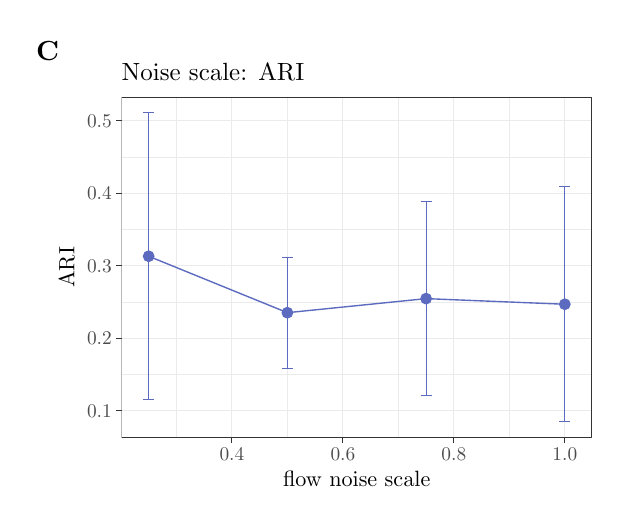
\begin{tikzpicture}[x=1pt,y=1pt]
\definecolor{fillColor}{RGB}{255,255,255}
\path[use as bounding box,fill=fillColor,fill opacity=0.00] (0,0) rectangle (206.87,171.36);
\begin{scope}
\path[clip] (  1.05,  1.87) rectangle (205.83,169.49);
\definecolor{drawColor}{RGB}{255,255,255}
\definecolor{fillColor}{RGB}{255,255,255}

\path[draw=drawColor,line width= 0.4pt,line join=round,line cap=round,fill=fillColor] (  1.05,  1.87) rectangle (205.83,169.49);
\end{scope}
\begin{scope}
\path[clip] ( 33.99, 23.34) rectangle (203.83,146.20);
\definecolor{fillColor}{RGB}{255,255,255}

\path[fill=fillColor] ( 33.99, 23.34) rectangle (203.83,146.20);
\definecolor{drawColor}{gray}{0.92}

\path[draw=drawColor,line width= 0.2pt,line join=round] ( 33.99, 46.05) --
	(203.83, 46.05);

\path[draw=drawColor,line width= 0.2pt,line join=round] ( 33.99, 72.25) --
	(203.83, 72.25);

\path[draw=drawColor,line width= 0.2pt,line join=round] ( 33.99, 98.45) --
	(203.83, 98.45);

\path[draw=drawColor,line width= 0.2pt,line join=round] ( 33.99,124.64) --
	(203.83,124.64);

\path[draw=drawColor,line width= 0.2pt,line join=round] ( 53.74, 23.34) --
	( 53.74,146.20);

\path[draw=drawColor,line width= 0.2pt,line join=round] ( 93.84, 23.34) --
	( 93.84,146.20);

\path[draw=drawColor,line width= 0.2pt,line join=round] (133.95, 23.34) --
	(133.95,146.20);

\path[draw=drawColor,line width= 0.2pt,line join=round] (174.05, 23.34) --
	(174.05,146.20);

\path[draw=drawColor,line width= 0.4pt,line join=round] ( 33.99, 32.95) --
	(203.83, 32.95);

\path[draw=drawColor,line width= 0.4pt,line join=round] ( 33.99, 59.15) --
	(203.83, 59.15);

\path[draw=drawColor,line width= 0.4pt,line join=round] ( 33.99, 85.35) --
	(203.83, 85.35);

\path[draw=drawColor,line width= 0.4pt,line join=round] ( 33.99,111.54) --
	(203.83,111.54);

\path[draw=drawColor,line width= 0.4pt,line join=round] ( 33.99,137.74) --
	(203.83,137.74);

\path[draw=drawColor,line width= 0.4pt,line join=round] ( 73.79, 23.34) --
	( 73.79,146.20);

\path[draw=drawColor,line width= 0.4pt,line join=round] (113.90, 23.34) --
	(113.90,146.20);

\path[draw=drawColor,line width= 0.4pt,line join=round] (154.00, 23.34) --
	(154.00,146.20);

\path[draw=drawColor,line width= 0.4pt,line join=round] (194.10, 23.34) --
	(194.10,146.20);
\definecolor{drawColor}{RGB}{92,107,192}

\path[draw=drawColor,line width= 0.5pt,line join=round] ( 43.72, 88.77) --
	( 93.84, 68.37) --
	(143.97, 73.45) --
	(194.10, 71.42);
\definecolor{fillColor}{RGB}{92,107,192}

\path[draw=drawColor,line width= 0.3pt,line join=round,line cap=round,fill=fillColor] ( 43.72, 88.77) circle (  1.97);

\path[draw=drawColor,line width= 0.3pt,line join=round,line cap=round,fill=fillColor] ( 93.84, 68.37) circle (  1.97);

\path[draw=drawColor,line width= 0.3pt,line join=round,line cap=round,fill=fillColor] (143.97, 73.45) circle (  1.97);

\path[draw=drawColor,line width= 0.3pt,line join=round,line cap=round,fill=fillColor] (194.10, 71.42) circle (  1.97);

\path[draw=drawColor,line width= 0.3pt,line join=round] ( 41.71,140.61) --
	( 45.72,140.61);

\path[draw=drawColor,line width= 0.3pt,line join=round] ( 43.72,140.61) --
	( 43.72, 36.92);

\path[draw=drawColor,line width= 0.3pt,line join=round] ( 41.71, 36.92) --
	( 45.72, 36.92);

\path[draw=drawColor,line width= 0.3pt,line join=round] ( 91.84, 88.33) --
	( 95.85, 88.33);

\path[draw=drawColor,line width= 0.3pt,line join=round] ( 93.84, 88.33) --
	( 93.84, 48.40);

\path[draw=drawColor,line width= 0.3pt,line join=round] ( 91.84, 48.40) --
	( 95.85, 48.40);

\path[draw=drawColor,line width= 0.3pt,line join=round] (141.97,108.47) --
	(145.98,108.47);

\path[draw=drawColor,line width= 0.3pt,line join=round] (143.97,108.47) --
	(143.97, 38.43);

\path[draw=drawColor,line width= 0.3pt,line join=round] (141.97, 38.43) --
	(145.98, 38.43);

\path[draw=drawColor,line width= 0.3pt,line join=round] (192.10,113.92) --
	(196.11,113.92);

\path[draw=drawColor,line width= 0.3pt,line join=round] (194.10,113.92) --
	(194.10, 28.92);

\path[draw=drawColor,line width= 0.3pt,line join=round] (192.10, 28.92) --
	(196.11, 28.92);
\definecolor{drawColor}{gray}{0.20}

\path[draw=drawColor,line width= 0.4pt,line join=round,line cap=round] ( 33.99, 23.34) rectangle (203.83,146.20);
\end{scope}
\begin{scope}
\path[clip] (  0.00,  0.00) rectangle (206.87,171.36);
\definecolor{drawColor}{gray}{0.30}

\node[text=drawColor,anchor=base east,inner sep=0pt, outer sep=0pt, scale=  0.70] at ( 30.39, 30.54) {0.1};

\node[text=drawColor,anchor=base east,inner sep=0pt, outer sep=0pt, scale=  0.70] at ( 30.39, 56.74) {0.2};

\node[text=drawColor,anchor=base east,inner sep=0pt, outer sep=0pt, scale=  0.70] at ( 30.39, 82.94) {0.3};

\node[text=drawColor,anchor=base east,inner sep=0pt, outer sep=0pt, scale=  0.70] at ( 30.39,109.13) {0.4};

\node[text=drawColor,anchor=base east,inner sep=0pt, outer sep=0pt, scale=  0.70] at ( 30.39,135.33) {0.5};
\end{scope}
\begin{scope}
\path[clip] (  0.00,  0.00) rectangle (206.87,171.36);
\definecolor{drawColor}{gray}{0.20}

\path[draw=drawColor,line width= 0.4pt,line join=round] ( 31.99, 32.95) --
	( 33.99, 32.95);

\path[draw=drawColor,line width= 0.4pt,line join=round] ( 31.99, 59.15) --
	( 33.99, 59.15);

\path[draw=drawColor,line width= 0.4pt,line join=round] ( 31.99, 85.35) --
	( 33.99, 85.35);

\path[draw=drawColor,line width= 0.4pt,line join=round] ( 31.99,111.54) --
	( 33.99,111.54);

\path[draw=drawColor,line width= 0.4pt,line join=round] ( 31.99,137.74) --
	( 33.99,137.74);
\end{scope}
\begin{scope}
\path[clip] (  0.00,  0.00) rectangle (206.87,171.36);
\definecolor{drawColor}{gray}{0.20}

\path[draw=drawColor,line width= 0.4pt,line join=round] ( 73.79, 21.34) --
	( 73.79, 23.34);

\path[draw=drawColor,line width= 0.4pt,line join=round] (113.90, 21.34) --
	(113.90, 23.34);

\path[draw=drawColor,line width= 0.4pt,line join=round] (154.00, 21.34) --
	(154.00, 23.34);

\path[draw=drawColor,line width= 0.4pt,line join=round] (194.10, 21.34) --
	(194.10, 23.34);
\end{scope}
\begin{scope}
\path[clip] (  0.00,  0.00) rectangle (206.87,171.36);
\definecolor{drawColor}{gray}{0.30}

\node[text=drawColor,anchor=base,inner sep=0pt, outer sep=0pt, scale=  0.70] at ( 73.79, 14.92) {0.4};

\node[text=drawColor,anchor=base,inner sep=0pt, outer sep=0pt, scale=  0.70] at (113.90, 14.92) {0.6};

\node[text=drawColor,anchor=base,inner sep=0pt, outer sep=0pt, scale=  0.70] at (154.00, 14.92) {0.8};

\node[text=drawColor,anchor=base,inner sep=0pt, outer sep=0pt, scale=  0.70] at (194.10, 14.92) {1.0};
\end{scope}
\begin{scope}
\path[clip] (  0.00,  0.00) rectangle (206.87,171.36);
\definecolor{drawColor}{RGB}{0,0,0}

\node[text=drawColor,anchor=base,inner sep=0pt, outer sep=0pt, scale=  0.80] at (118.91,  5.64) {flow noise scale};
\end{scope}
\begin{scope}
\path[clip] (  0.00,  0.00) rectangle (206.87,171.36);
\definecolor{drawColor}{RGB}{0,0,0}

\node[text=drawColor,rotate= 90.00,anchor=base,inner sep=0pt, outer sep=0pt, scale=  0.80] at ( 16.86, 84.77) {ARI};
\end{scope}
\begin{scope}
\path[clip] (  0.00,  0.00) rectangle (206.87,171.36);
\definecolor{drawColor}{RGB}{0,0,0}

\node[text=drawColor,anchor=base west,inner sep=0pt, outer sep=0pt, scale=  0.90] at ( 33.99,152.18) {Noise scale: ARI};
\end{scope}
\begin{scope}
\path[clip] (  0.00,  0.00) rectangle (206.87,171.36);
\definecolor{drawColor}{RGB}{0,0,0}

\node[text=drawColor,anchor=base,inner sep=0pt, outer sep=0pt, scale=  1.00] at (  7.20,159.49) {\bfseries C};
\end{scope}
\end{tikzpicture}
